\documentclass[a4paper,12pt]{article}
\usepackage{amssymb}
\usepackage{amsmath}
\usepackage{graphicx}
\usepackage{float}
\usepackage{subfigure}
\usepackage{geometry}
\pagestyle{plain}
\usepackage{listings} 
\usepackage{multirow}
\geometry{left=2.2cm, right=2.2cm, top=3cm, bottom=3cm}
\usepackage{algorithm}  
\usepackage{algpseudocode}   
\renewcommand{\algorithmicrequire}{\textbf{Input:}} 
\renewcommand{\algorithmicensure}{\textbf{Output:}}

\title{A Bayesian Perspective on Distributional Deep Q-Learning}
\date{\today}

\author{Ni Chengzhuo\footnote{This is the homework for the course Bayesian Theory and Computation.}\\
1500011343\\
School of Mathematical Science, Peking University\\
}

\usepackage{cite}
\begin{document}
\maketitle

\abstract{We propose a Bayesian framework for Q-value estimation. We utilize the Bayesian neural network to form a posterior distribution of the Q-value given the historical data. Under this framework, both the action and the estimation of the target value can be sampled from the posterior distribution, which allows for a more robust estimation as well as encouraging exploration. We show that using the posterior mean of the Bayesian Q-value distribution, rather than a deterministic network, improves the stability and performance of Q-Learning methods in several platforms.}

\section{Introduction}
One of the primary goals of artificial intelligence is to solve complex tasks from unprocessed, high-dimensional input. Recently, significant progress has been made combining advances in deep learning with reinforcement learning, resulting in the ``Deep Q Network'' (DQN)\cite{DQN} algorithm and its variations\cite{DDQN, PDQN, DuelDQN} that are capable of human level performance on many platforms. 

However, as these methods usually deal with unstable environments with high variance, distributional perspectives of function approximations have begun to gain popularity.  Currently, such methods typically use many approximators to fit a distribution\cite{DisDQN, BDQN}. However, recent advances in Bayesian inference using deep neural networks have been successful in providing estimates with uncertainty\cite{Dropout, BNN, BNN2, BNN3}. Another problem in RL is the exploration-exploitation problem, which has become a main focus for researchers nowadays. One effective solution to the problem is the Thompson Sampling Method\cite{TS, TS2, TS3}, whose exploration strategy is based on the posterior distribution of the model parameters. However, since calculating the posterior is usually intractable for complex models (e.g. neural network), the method has not been widely applied in deep reinforcement learning so far.

In this work, we develop an approach where a Bayesian neural network (BNN) is utilized as a Q-value function approximator in Deep Q-Learning. We apply several methods\cite{BNN, Dropout} from previous work to get an approximate posterior distribution of the network weights and then form a posterior distribution of the Q-value estimation. With this estimated distribution, we develop a distributional perspective on Q-Learning that is different from the previous work\cite{DisDQN}. Based on our structure, we are also able to apply the Thompson Sampling method, which is shown to be more effective when compared to other exploration strategies such as $\epsilon$-greedy or Boltzmann method. We demonstrate the significance of using Bayesian method across a range of Q-Learning methods including DQN, Double DQN, DQN with prioritized replay memory on several toy platforms.  

\section{Background and related work}
\subsection{Reinforcement Learning Background}
In the standard reinforcement learning setting, an agent interacts with an environment over a number of time steps. At each time step $t$, the agent receives a state $s_t$ and selects an action $a_t$ from a set of possible actions $\mathcal{A}$ according to its policy $\pi$. Then the agent receives the next state $s_{t+1}$ and a scalar reward $r_t$. The process continues until the terminal state is reached. The return $Z_t = \sum_{k=0}^\infty \gamma^kr^{t+k}$ is the discounted accumulated reward from time step $t$ with discount factor $\gamma \in (0, 1]$. The goal of the agent is to maximize the expected return from each state $s_t$. 

The Q-value $Q^{\pi}(s, a) = \mathbb{E}[Z_t|s, a]$ is the expected return for selecting action $a$ in state $s$ and following policy $\pi$ afterwards. The optimal Q-value $Q^*(s,a) =\max_\pi Q^\pi(s,a)$ is the maximum value for state $s$ and action $a$ achievable by any policy. In DQN, the policiy $\pi(s, a)$ and the value function $Q(s, a)$ are represented with deep neural networks. At each step, given the current state, the agent selects an action $\epsilon$-greedily according to the action values, and adds the transition $(s_t , a_t , r_t, S_{t+1})$ to a replay buffer. The parameters of the neural network are optimized using stochastic gradient descent to minimize the loss

\begin{equation}
L = \mathbb{E}(r_t +\gamma \max_{a'}Q_{\bar{\theta}}(s_{t+1},a')-Q_\theta(s_t,a_t))^2
\end{equation}

In practice, the optimization is performed on mini batches sampled from the replay buffer. 

\subsection{Distributional Perspectives in RL}
Several recent works have investigated the distributional perspectives in reinforcement learning. In \cite{BAC}, a Bayesian framework was applied to the actor-critic architecture by fitting a Gaussian Process (GP) for the critic which allowed for a closed-form derivation of update rules. In \cite{Dropout}, dropout uncertainty estimates of a Q-value function were used for Thompson sampling and optimistic exploration. In \cite{DisDQN}, both the structure and the update rule of the value function are based on a distributional perspective. Similarly, in \cite{BDQN}, the authors use k-heads on the Q-value to model a distribution rather than the dropout approach of \cite{Dropout}. 

Here we use the Bayesian method to build a posterior distribution for the Q-value, which is similar to the work of \cite{BAC}, but we apply the procedure to the Q-learning framework rather than the actor-critic framework. Also, we build our model via a more complicated neural network rather than the relatively simple Gaussian Process, which is capable to fit more complex distributions. 

\subsection{Bayesian Neural Network}
Given training inputs $X = \{x_1, \cdots , x_N\}$ and their outputs $Y = \{y_1 , \cdots, y_N\}$, in the Bayesian framework we would like to infer a distribution over parameters $w$ of a function $y = f^w(x)$ that could have generated the outputs. Following the Bayesian approach, we first put some prior distribution over the parameters $p_0(w)$. We further need to define a likelihood over the outputs given the inputs $p(y|x, w)$, which is usually assumed to be a softmax function for classification or a Gaussian distribution for regression. Given a dataset $X, Y$, we then look for the posterior distribution of the parameters: $p(w|X, Y)$. With it we can predict an output for a new input point $x^∗$ by integrating

\begin{equation}
p(y^* | x^*, X, Y) = \int p(y^*|x^*, w)p(w|X, Y)dw
\end{equation}

When the prior distribution is placed on a neural network's weights $w = \{W_i\}^L_{i=1}$ , the model is called a Bayesian neural network(BNN). In practice, given weight matrices $W_i$ at layer $i$, we often place Gaussian prior distributions over the weights, i.e., $p_0(W_i) = N (W_i ; 0, \sigma^2 I)$. Under this setting, both the parameters and the predictions of the network turn from deterministic values into variables from specific distributions. A comparison between the usual neural network and the Bayes neural network is shown in the following figure, 

\begin{figure}[htb!]
\center
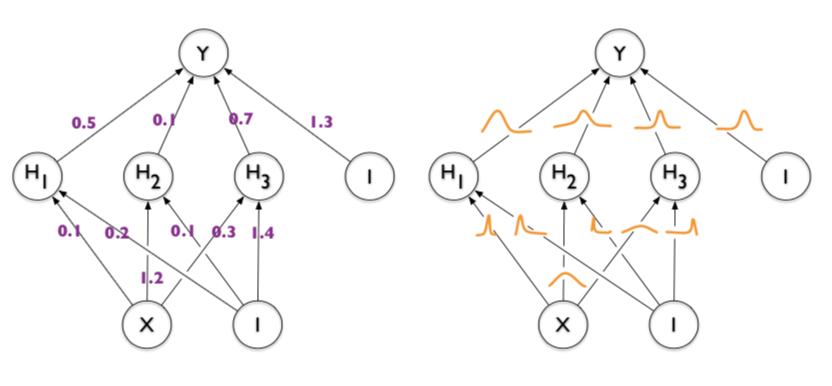
\includegraphics[scale=0.6]{bnn}
\caption{Left: each weight has a fixed value. Right: each weight is assigned a distribution.}
\end{figure}

\section{A Bayesian Perspective on Q-learning}
\subsection{The Bayesian Estimation of Q-value}
In the previous setting of Q-learning, the Q-value $Q^w(s_t, a_t)$ is a deterministic function parameterized by $w$ which estimates the expectation of the return $Z_t$. This deterministic output version is not compatible with the Bayesian method, since a likelihood is needed to compute a posterior distribution over the weights, which becomes a tricky delta function $\delta_{x^*}(\cdot)$ in the deterministic case. To apply the Bayesian method, the output of the Q-value function must first be modified from a single expectation value to a distributional estimation for $Z_t$, 

\begin{equation}
z_t \sim p(\cdot | s_t, a_t, w)
\end{equation}

where $p(\cdot | s_t, a_t, w)$ is the c.d.f. of a continuous probability distribution parameterized by $w$. Clearly, $p(z | s_t, a_t, w)$ is the likelihood of $z$ when the parameter of the model is $w$ and the current state and action are $s_t$ and $a_t$, respectively. Suppose we have got a number of state-action pairs $\{(s_t, a_t)\}_{t=1}^T$ and their corresponding return $\{z_t\}_{t=1}^T$, and we denote the data we have got so far as $\mathcal{D} = {(s_t, a_t, z_t)}_{t=1}^T$. We further assume that the returns are independent between different time steps, then the likelihood of the whole data can be computed as below, 

\begin{equation}
p(\mathcal{D} | w) = \prod_{t=1}^T p(z_t | s_t, a_t, w)
\end{equation}

In the frequentists' perspective, as the problem is usually handled before, the true value of $w$ exists which is usually estimated by the maximum likelihood estimation(MLE) method, 

\begin{equation}
\hat{w} = \textrm{argmax}_w p(\mathcal{D} | w) =\textrm{argmax}_w\prod_{t=1}^T p(z_t | s_t, a_t, w)
\end{equation}

When the likelihood is assumed to be in the form of a Gaussian distribution, the above problem is equivalent to finding the minimizer of the mean squared loss, 

\begin{equation}
\hat{w} = \textrm{argmin}_w \frac{1}{T}\sum_{t=1}^T (z_t - \mu_t(s_t, a_t, w))^2
\end{equation}

However, when the problem is looked into with a Bayesian perspective, where a prior $p(w)$ is usually placed over the parameter $w$, the parameter is assumed to be a random variable which can only be estimated via the posterior distribution, 

\begin{equation}
\hat{w} \sim p(w | \mathcal{D}) \sim p(\mathcal{D} | w)p(w)
\end{equation}

when the posterior of $w$ is given, the posterior estimation of the return of some new state-action pair $(s, a)$ can be got by the following equation,

\begin{displaymath}
z \sim \int p(z | s, a, w)p(w | \mathcal{D}) dw
\end{displaymath}

To estimate the Q-value $\hat{q}$, the posterior expectation of $z$ is calculated via integration,  

\begin{equation}
\hat{q} = \iint zp(z | s, a, w)p(w | \mathcal{D}) dwdz
\end{equation}

 In practice, however, the integral is usually hard to calculate. One solution to the problem is to first sample several $z$ from the posterior distribution, and replace the estimation by an empirical mean. But due to the randomness in $w$ and the complicated structure in neural network, it is still intractable to sample $z$ directly from its distribution. Therefore, we must sample $w$ as well, i.e., we first sample several $\{w_i\}_{i=1}^k \sim f(w | \mathcal{D})$ from the posterior distribution, then for each $w_i$, we get the mean value of the discounted cumulative rewards $\{\bar{z}_i\}_{j=1}^l$ from the c.d.f. $p(z | s, a, w_i)$, then the mean value can be estimated as  

\begin{equation}
\hat{q}(s, a) = \frac{1}{k}\sum_{i=1}^k \bar{z}_i
\end{equation}

\subsection{Action Selection with Thompson Sampling Method}
In the previous Q-learning process, the action is selected $\epsilon$-greedily to be the one which maximizes the Q-value under the current state. 

\begin{equation}
a_t = \textrm{argmax}_a \hat{q}(s_t, a)
\end{equation}

However, the above strategy has several weaknesses. The $\epsilon$-greedy strategy is shown to be insufficient for exploration in practice, and it is costly to calculate the posterior mean under the Bayesian setting. To achieve better exploration and reduce the cost, we instead use the Thompson sampling method. At each step, we first sample the weight $w_t$ from the current posterior $w_t \sim f(w | \mathcal{D}_t)$, then we choose the action $a_t$ to be the maximizer for the Q-value estimation under $w_t$, 

\begin{equation}
a_t = \textrm{argmax}_a \bar{z}(s_t, a | w_t)
\end{equation}

The basic framework of the Thompson sampling method is written in the pseudocode below, 

\begin{algorithm}[htb]
\begin{algorithmic}[1]
\caption{The Thompson sampling method}
\Require the posterior distribution $p(w | \mathcal{D})$, the likelihood function $p(\cdot | w)$, the current state $s$
\Ensure the selected action $a^*$
\State Sample $w$ from $p(w | \mathcal{D})$
\State Calculate $\bar{z}(s, a) = \mathbb{E}[z | s, a, w]$ for each $a\in\mathcal{A}$
\State Return $a^* = \textrm{argmax}_a\bar{z}(s, a)$ 
\end{algorithmic}
\end{algorithm}


\section{Implement the Bayesian Model}
To implement a specific update rule for the Bayesian network, we propose two methods, the first one based on the variational inference method while the second one applying a simpler procedure with a perspective related to the dropout method. 

\subsection{Variational Inference Under Gaussian approximation}
\subsubsection{Variational Inference}
In practice, it is intractable to get an explicit expression for the posterior distribution of the network weights. One alternative way is to use the variational inference method to simplify calculation. Variational inference finds the parameters $\theta$ of a distribution on the weights $q(w|\theta)$ that minimises the Kullback-Leibler (KL) divergence with the true Bayesian posterior on the weights,

\begin{equation}
\begin{aligned}
\theta^* &= \textrm{argmin}_\theta \textrm{KL}[q(w|\theta)||p(w|\mathcal{D})]\\
& = \textrm{argmin}_\theta \int q(w|\theta)\ln \frac{q(w|\theta)}{p(w | \mathcal{D})p(w)}\\
& =  \textrm{argmin}_\theta \textrm{KL} [q(w|\theta) ||  p(w)] - \mathbb{E}_{q(w|\theta)} [\ln p(\mathcal{D}|w)]
\end{aligned}
\end{equation}

The resulting cost function is variously known as the variational free energy or the expected lower bound. We suppose $q(w | \theta)$ takes the simple form of independent Gaussian distribution where $\theta = (\mu, \rho)$ and the Gaussian distribution takes the form $w\sim N(\mu, \ln^2(1 + \exp(\rho)))$. The main procedure to update procedure is based on one conclusion proposed in \cite{BNN}. 

\paragraph{Proposition 1.}
Let $\varepsilon$ be a random variable having a probability density given by $q(\varepsilon)$ and let $w = t(\theta,\varepsilon)$ where $t(\theta,\varepsilon)$ is a deterministic function. Suppose further that the marginal probability density of $w, q(w|\theta)$, is such that $q(\varepsilon)d\varepsilon = q(w|\theta)dw$. Then for a function f with derivatives in $w$:

\begin{displaymath}
\frac{\partial}{\partial\theta}\mathbb{E}_{q(w|\theta)}[f(w, \theta)] =  \mathbb{E}_{q(\varepsilon)}\left[\frac{\partial f(w, \theta)}{\partial w}\frac{\partial w}{\partial\theta} + \frac{\partial f(w, \theta)}{\partial\theta}\right]
\end{displaymath}

According to this proposition, $\theta$ can be updated by first sampling $w$ from its corresponding distribution and then use the ordinary gradient descent method to update its parameters, which leads to the following procedure, 

\begin{algorithm}[htb]
\begin{algorithmic}[1]
\caption{Updating procedure for $\theta=(\mu,\rho)$}
\Require the data $\mathcal{D}$,  the initial point $(\mu,\rho)$, the learning rate $r$
\State Sample $\varepsilon\sim N(0,I)$
\State Let $w=\mu + \ln(1+\exp(\rho))\odot \varepsilon$
\State Let $f(w,\mu,\rho)=\ln q(w|\mu,\rho)-\ln p(w)p(\mathcal{D}|w)$
\State Calculate the gradient with respect to the mean
\begin{displaymath}
\Delta_\mu = \frac{\partial f(w,\mu,\rho)}{\partial w} + \frac{\partial f(w,\mu,\rho)}{\partial \mu}
\end{displaymath}
\State Calculate the gradient with respect to the standard deviation parameter $\rho$
\begin{displaymath}
\Delta_\rho = \frac{\partial f(w,\mu,\rho)}{\partial w}\frac{\varepsilon}{1 + \exp(-\rho)} + \frac{\partial f(w,\mu,\rho)}{\partial \rho}
\end{displaymath}
\State Update the variational parameters
\begin{displaymath}
\begin{aligned}
\mu &= \mu - r\Delta\mu\\
\rho &= \rho - r\Delta\rho
\end{aligned}
\end{displaymath}
\end{algorithmic}
\end{algorithm}

\subsubsection{Compute the target value}
An widely applied way for target estimation in Q-learning is the bootstrap method, which estimates the current Q-value via the current reward and an estimation of the return of next state, 

\begin{equation}
z^{\textrm{target}}_t = r_t + \gamma \max_a\hat{z}(s_{t+1}, a)
\end{equation}

Here the equation means that the LHS and RHS are identically distributed. To sample from the right hand expression, we first sample the weight $w$ from the posterior distribution and calculate $\max_a\hat{z}(s_{t+1}, a, w)$. The target estimation is then written as below, 

\begin{equation}
z^{\textrm{target}}_t = r_t + \max_a\hat{z}(s_{t+1}, a, w)
\end{equation}

After we have got the target value, the pair $(s_t, a_t, y_{\textrm{targ}})$ is added into the historical dataset to update the posterior distribution. 

\subsubsection{Assumption on the likelihood and prior}
Like many previous methods, we assume that the likelihood for $z_t$ given $s_t, a_t$ and $w$ takes the form of Gaussian distribution. Meanwhile, the prior on the weights is also set to be an independent Gaussian distribution with equal variance for each component. The above assumptions lead to an explicit expression on the target loss of the variational method, 

\begin{equation}
\begin{aligned}
f(w, \mu, \rho) &= \ln q(w | \mu, \rho) - \ln p(\mathcal{D}|w)\ln p(w)\\
&\sim -\frac{1}{2}1^T\ln\sigma - \frac{(w - \mu)^T(w - \mu)}{2\sigma^2}+\frac{\alpha}{2T} \sum_{t=1}^T(\hat{z}(s_t, a_t, w)-z^{\textrm{target}}_t)^2 + \frac{\beta}{2} w^Tw 
\end{aligned}
\end{equation}

where $\alpha > 0, \beta > 0$ are different hyperparameters associated to the variance of these distributions and $\sigma= \ln(1 + \exp(\rho))$ is the standard error of $w$. Under this setting, we can write $\Delta_\mu, \Delta_\rho$ explicitly, 

\begin{equation}
\Delta_\mu = \alpha\frac{\sum_{t=1}^T(\hat{z}(s_t, a_t, w)-z^{\textrm{target}}_t)}{T}\frac{\partial \hat{z}(s_t, a_t, w)}{\partial w} + \beta w - \frac{\mu - w}{\ln^2(1 + \exp(\rho))}\\
\end{equation}

\begin{equation}
\begin{split}
\Delta_\rho = \left(\alpha\varepsilon\odot\frac{\sum_{t=1}^T(\hat{z}(s_t, a_t, w)-z^{\textrm{target}}_t)}{T}\frac{\partial \hat{z}(s_t, a_t, w)}{\partial w} + \beta\varepsilon\odot w - \frac{1}{\ln(1 + \exp(\rho))} +  \frac{(w - \mu)^T(w - \mu)}{\ln^3(1 + \exp(\rho))} \right) \\
\odot\frac{1}{1 + \exp(-\rho)}
\end{split}
\end{equation}

\subsection{Dropout as a Bayesian Approximation}
In \cite{Dropout}, the authors propose a different viewpoint on posterior calculation, which results in a simpler procedure than the previous work. In this work, the authors assume that the approximator of the intractable posterior $q(w)$ is a distribution over matrices whose columns are randomly set to zero, 

\begin{equation}
\begin{aligned}
W_i&=M_i\textrm{diag}([z_{i,j}]_{j=1}^{K_i})\\
z_{i,j} &\sim \textrm{Bernoulli}(p_i) \textrm{ for } i=1, \cdots, L, j = 1,\cdots, K_{i-1}
\end{aligned}
\end{equation}

given some probabilities $p_i$ and matrices $M_i$ as variational parameters. The objective function is then estimated by Monte Carlo integration with a single sample $\hat{w}_n \sim q(w)$ to get an unbiased estimate $-\ln p(y_n |x_n , \hat{w}_n)$. After some scaling, the estimated objective function can be written as, 

\begin{equation}
\begin{aligned}
L \propto -\frac{1}{N}\sum_{n=1}^N\ln p(y_n|x_n,\hat{w}_n) + \frac{1}{2N}\sum_{i=1}^L(p_il^2\Vert M_i\Vert_2^2 + l^2\Vert m_i\Vert_2^2)
\end{aligned}
\end{equation}

which is exactly the same with minimization objective in dropout, 

\begin{equation}
\begin{aligned}
L=\frac{1}{N}\sum_{i=1}^N E(y_i,\hat{y}_i)+ \lambda\sum_{i=1}^L(\Vert W_i \Vert_2^2 + \Vert b_i\Vert_2^2) 
\end{aligned}
\end{equation}

Under this setting, getting the sampled Q-value with a sampled $\hat{w}$ from $q(w)$ is equivalent to applying the dropout method directly during the forward propagation, and the weights of the network can be updated in the same way as in the dropout method. 

\section{Experiments}
The algorithm is applied on several toy environments. We compare the outcome of our algorithm with some previous proposed Q-learning algorithms\footnote{Codes available at https://github.com/hzxsnczpku/banrinochoujou}, our experiments are aimed to answer the following two questions, 

\begin{itemize}
\item[-] Is the Thompson Sampling method helpful for efficient exploration?
\item[-] Can the Bayesian neural network outperform the previous algorithms under our environments?
\end{itemize}

\subsection{N-Chains}
We first test the methods in the environment called nChain. Under this environment, the agent starts at position 1, and at each step, the agent can choose to move one step forward or one step backward. When the agent reaches position 0, the game is ended and the agent receives a reward of 1. When the agent reaches position n, the game is also ended and the agent receives a reward of n. The aim of the agent is to receive a reward as high as possible throughout one game, which can be achieved if the agent always chooses to move forward. However, to achieve this, the agent needs to explore for a long time since there is no reward until the final state is reached. We calculate the mean episode reward between episode 90-110 under different algorithms and different chain lengths. The result is recorded in table 1. From the result we can see, the Bayesian method improves the performance of the agent, which shows that the Thompson sampling method can encourage efficient exploration under certain environments. 

\begin{figure}[htb!]
\center
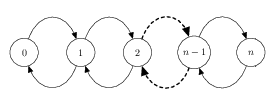
\includegraphics[scale=0.85]{nchain_demo}
\caption{A demo of the nChain environment. }
\end{figure}

\begin{table}[htb!]
\center
\caption{Mean episode reward between episode 90-110 under different algorithms and different chain lengths}
\begin{tabular}{c | c c c c c}
\hline
N & 20 & 30 & 50 & 80 & 100\\
\hline
Bayesian TS & \textbf{20.0} & 14.05 & \textbf{50.0} & \textbf{80.0} & 80.15\\
Bayesian Dropout & 19.05 & \textbf{30.00} & 45.10 & 76.05 & \textbf{80.20}\\
DQN no noise  & 14.30 & 6.00 & 15.50 & 4.00 & 60.00\\
DQN $\varepsilon$-greedy & 9.00 & 9.05 & 10.35 & 24.25 & 40.25\\
\hline
\end{tabular}
\end{table}

\subsection{Classical Control}
We further test our method on two classical control problems. The environments are the CartPole-v0 and the Acrobot-v1, respectively. In the first environment, the goal is to keep  the pole on a cart standing as long as possible. In the second environment, the goal is to make the end of the pole touch a horizontal line as quickly as possible. In both two environments, the state space is a two dimensional continuous vector and the action is an integer taking value in $\{0, 1\}$. We test two versions of posterior updater of the Bayesian method, the first one of which is utilizing the variational inference with Gaussian approximator to the posterior while the second one is applying directly the dropout method.  The original DQN algorithm with and without $\epsilon$-greedy exploration strategy are tested as baselines. The double DQN algorithm and DQN with a prioritized replay memory are also tested. 

\begin{figure}[htb!]
\center
\includegraphics[height=4cm]{Cartpole_sample}
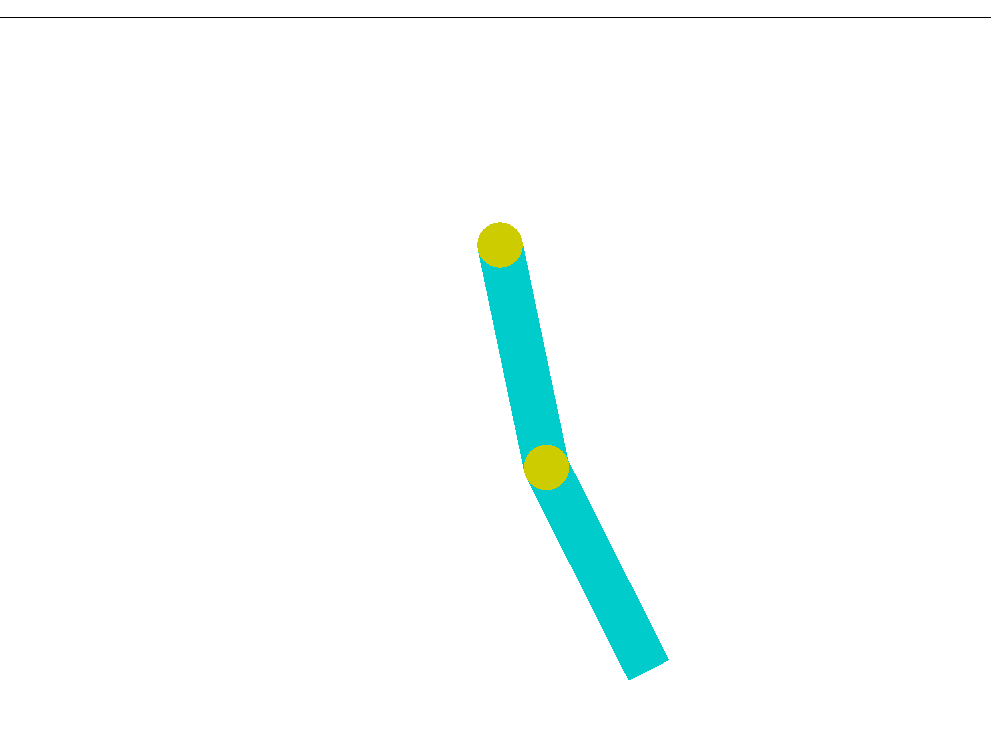
\includegraphics[height=4cm]{Acrobot_sample}
\caption{Left: A demo of the CartPole environment. Right: A demo of the Acrobot environment. }
\end{figure}

We plot the episode rewards of different algorithms performed in the two platforms at the following two figures, where each reward is smoothed as the mean reward of the nearby 10 episodes and the shadow area covers two times of standard error. 

\begin{figure}[htb!]
\center
\includegraphics[height=5cm]{CartPole}
\includegraphics[height=5cm]{Acrobot}
\caption{Left: Experimental results on the CartPole environment, where the score is smoothed over a number of episodes.  Right: Experimental results on the Acrobot environment, where the score is smoothed over a number of episodes. }
\end{figure}

In both two environments, the agent behaves poorly when no exploration strategy is applied, staying at a low score for a very long time. We can see from our results that the Bayesian estimation with variational inference method achieves the best performance, which outperforms all of the other algorithms at the very beginning of the CartPole platform and is slightly better than the other algorithms at the Acrobot environment. One of our findings is that this method gets a higher score even at the beginning of the game, where the strategy is nearly random. This fact shows that the variational inference method combined with Thompson Sampling method achieves very high exploring efficiency. The dropout method behaves very similar to the previous Q-learning methods, but the result is still inspiring since it means that we have found a new method which is at least not worse than the existing methods. 

\section{Conclusion and further work}
We use the Bayesian method to model the distribution of the return in Q-learning using the variational inference method and as well as the dropout-as-Bayesian-approximation method. We apply the Thompson sampling method given the posterior distribution of the parameters and show that the method achieves a better performance than the previous algorithms in several platforms. However, we find that our methods can sometimes be unstable and have a higher computation cost than the previous algorithms, which leads to the poor performance of our algorithms under some more complicated environments. Further works include but are not limited in improving the stability of the algorithms, cutting down the computation cost, doing experiments on some more complicated environments, etc.

\begin{thebibliography}{99}
	\bibitem{DQN}
	Mnih V, Kavukcuoglu K, Silver D, et al. Playing atari with deep reinforcement learning[J]. arXiv preprint arXiv:1312.5602, 2013.
	\bibitem{DDQN}
	Van Hasselt H, Guez A, Silver D. Deep Reinforcement Learning with Double Q-Learning[C]//AAAI. 2016: 2094-2100.
	\bibitem{PDQN}
	Schaul T, Quan J, Antonoglou I, et al. Prioritized experience replay[J]. arXiv preprint arXiv:1511.05952, 2015.
	\bibitem{DuelDQN}
	Wang Z, Schaul T, Hessel M, et al. Dueling network architectures for deep reinforcement learning[J]. arXiv preprint arXiv:1511.06581, 2015.
	\bibitem{DisDQN}
	Marc G Bellemare, Will Dabney, and Rémi Munos. A distributional perspective on reinforcement learning. arXiv preprint arXiv:1707.06887, 2017.
	\bibitem{BDQN}
	Ian Osband, Charles Blundell, Alexander Pritzel, and Benjamin Van Roy. Deep exploration via bootstrapped DQN. In Advances in Neural Information Processing Systems, pages 4026–4034, 2016.
	\bibitem{Dropout}
	Yarin Gal and Zoubin Ghahramani. Dropout as a bayesian approximation: Representing model uncertainty in deep learning. In international conference on machine learning, pages 1050–1059, 2016.
	\bibitem{BNN}
	Charles Blundell, Julien Cornebise, Koray Kavukcuoglu, and Daan Wierstra. Weight uncertainty in neural networks. arXiv preprint arXiv:1505.05424, 2015.
	\bibitem{BNN2}
	José Miguel Hernández-Lobato and Ryan P. Adams. Probabilistic backpropagation for scalable learning of bayesian neural networks. In Proceedings of the 32nd International Conference on Machine Learning (ICML), pages 1861–1869, 2015.
	\bibitem{BNN3}
	David Krueger, Chin-Wei Huang, Riashat Islam, Ryan Turner, Alexandre Lacoste, and Aaron Courville. Bayesian hypernetworks. arXiv preprint arXiv:1710.04759, 2017.
	\bibitem{TS}
	Agrawal S, Goyal N. Analysis of Thompson sampling for the multi-armed bandit problem[C]//Conference on Learning Theory. 2012: 39.1-39.26.
	\bibitem{TS2}
	Chapelle O, Li L. An empirical evaluation of thompson sampling[C]//Advances in neural information processing systems. 2011: 2249-2257.
	\bibitem{TS3}
	Kaufmann E, Korda N, Munos R. Thompson Sampling: An Asymptotically Optimal Finite-Time Analysis[C]//ALT. 2012, 12: 199-213.
	\bibitem{BAC}
	Mohammad Ghavamzadeh, Yaakov Engel, and Michal Valko. Bayesian policy gradient and actor-critic algorithms. Journal of Machine Learning Research, 17(66):1–53, 2016.
	\bibitem{RL}
	Sutton R S, Barto A G. Reinforcement learning: An introduction[M]. Cambridge: MIT press, 1998.
	\bibitem{DL}
	LeCun Y, Bengio Y, Hinton G. Deep learning[J]. Nature, 2015, 521(7553): 436-444.
\end{thebibliography}

\end{document}

